\section{Graphical Model Formulation}
\label{sec:model}
\begin{wrapfigure}{r}{0.25\textwidth}
\begin{center}
%\framebox[4.0in]{$\;$}
%\fbox{\rule[-.5cm]{0cm}{4cm} \rule[-.5cm]{4cm}{0cm}}
 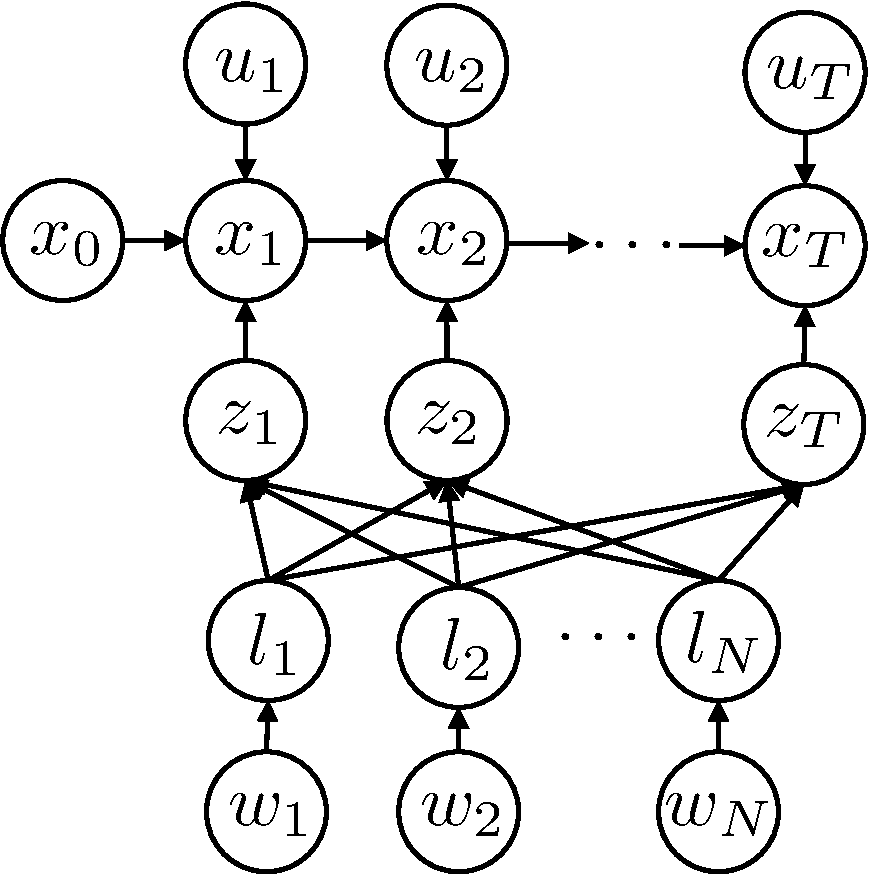
\includegraphics[width=0.25\textwidth]{fig/model} 
\end{center}
\caption{Graphical Model Formulation. Dark nodes are observed.}
\label{fig:model}
\end{wrapfigure}

Following \cite{isam} we formulate the SLAM problem in graphical models in Figure \ref{fig:model}. Specifically, the robot states are denoted by $X = \{x_i\}$ with $i \in 0, \dots T$, the landmarks by $L = \{l_j\}$ with $j \in 1,\dots, N$, the control inputs by $U = \{u_i\}$ for $i \in 1,\dots, T$ and the landmark measurements by $Z = \{z_k\}$ with $k \in 1, \dots, K$. In addition to the classical graph SLAM formulation, we also add latent parameters $W = \{w_j\}$ with $j \in 1, \dots, N$  The joint probability of all variables and measurements are given by
\begin{equation}
P(X, L, U, Z, W) \propto \prod\limits_{i}P(x_i|x_{i-1}, u_i)\prod\limits_{k}P(z_k|x_{i_k}, l_{j_k}, w_k).
\label{eq:jointProb}
\end{equation}

Then the maximum likelihood (ML) estimate of the unobserved poses $X$ and landmarks $L$ given observations $Z$ and known controls $U$ and the current latent parameters $W$ is
\begin{equation}
\hat{X}_{\mathrm{ML}}, \hat{L}_{\mathrm{ML}} = \operatorname*{arg\,max}_{X,L} P(X,L,U,Z,W).
\end{equation}
To calculate the ML estimate, the objective is converted into a nonlinear least
squares problem in this form $\operatorname*{arg\,min}_{\Delta \theta} || A
\Delta \theta  - b ||^2$ by algebraic manipulation, and then optimized using
different numeric methods. The detailed derivation is skipped here.

Using a Gaussian representation with the latent extension, the sensor
model, the process model and measurement equation follows
\begin{equation}
\begin{aligned}
x_i &= f_i(x_{i-1}, u_i) + \omega_i \\
z_k &= h_k(x_{i_k}, l_{j_k}) + \nu_k
\end{aligned}
\end{equation}
where $\omega_i$ and $\nu_k$ follow zero-mean normal distribution with covariance matrices $\Gamma_i$ and $\Sigma_k$. With this formulation, the second part of the equation \ref{eq:jointProb} is
\begin{equation}
P(z_k|x_{i_k}, l_{j_k}, w_k)\propto \exp\{-w_k((z_k - h_k(x_{i_k}, l_{j_k}))^T\Sigma_k^{-1}(z_k - h_k(x_{i_k}, l_{j_k}))\}.
\label{eq:sensor}
\end{equation}
$w_k$ is the likelihood that the measurement comes from static landmark. In our case, we need to infer what those values are and ideally the process could be online or folows an incremental fashion. Possible solutions could be 1) using visual cues to cluster the landmarks to ``moving''/``static''. Challenges mainly lies in whether the features we use is reliable or not in terms of this clustering task; 2) instead of using an expensive EM algorithm in \cite{rogers2010slam}, we design particle filters to incrementally update parameter $w_k$, making the whole process online.
